\documentclass[a4paper,twoside,zihao=5,UTF8]{ctexrep}

\ctexset{
	section = {
		format+ = \zihao{-4} \heiti \raggedright,
		name = {,、},
		number = \chinese{section},
		beforeskip = 1.0ex plus 0.2ex minus .2ex,
		afterskip = 1.0ex plus 0.2ex minus .2ex,
		aftername = \hspace{0pt}
	},
	subsection = {
		format+ = \zihao{5} \heiti \raggedright,
		name = {\thesubsection、},
		name = {,、},
		number = \arabic{subsection},
		beforeskip = 1.0ex plus 0.2ex minus .2ex,
		afterskip = 1.0ex plus 0.2ex minus .2ex,
		aftername = \hspace{0pt}
	}
}

\usepackage{titling}

\usepackage[utf8]{inputenc}
\usepackage[T1]{fontenc}

\usepackage{lmodern}
\usepackage{microtype}
\usepackage{blindtext}


\usepackage{listings}
\usepackage{xcolor}

\usepackage{geometry}
\geometry{left=2.3cm,right=2cm,top=2.5cm,bottom=2.0cm}

\usepackage{amsmath}
\usepackage{float}
\usepackage{hyperref}

\usepackage{graphics}
\usepackage{graphicx}

\usepackage{subfigure}
\usepackage{epsfig}
\usepackage{float}

\usepackage{algorithm}
\usepackage[noend]{algpseudocode}

\usepackage{booktabs}
\usepackage{threeparttable}
\usepackage{longtable}
\usepackage{listings}

% cite package, to clean up citations in the main text. Do not remove.
\usepackage{cite}

\usepackage{color,xcolor}

%% The amssymb package provides various useful mathematical symbols
\usepackage{amssymb}
%% The amsthm package provides extended theorem environments
\usepackage{amsthm}
\usepackage{amsfonts}
\usepackage{enumerate}
\usepackage{enumitem}
\usepackage{listings}

\usepackage{indentfirst}
\usepackage{setspace}
\usepackage{siunitx}

\newcommand{\subtitle}[1]{%
  \posttitle{%
    \par\end{center}
    \begin{center}\large#1\end{center}
    \vskip0.5em}%
}

%%%%%%%%%%%%%
\newcommand{\Authors}{熊恪峥 \ 徐昊 \ 陈奕凝}  % Replace your name here
\newcommand{\BookTitle}{以Transformer为主干网络的遥感图像分割}  % Change your paper title here
\newcommand{\BookSubtitle}{基于ST-UNet} % Replace the type of your report here
\newcommand{\Date}{2022年5月4日}
%%%%%%%%%%%%%

\lstset{
	basicstyle          =   \sffamily,          % 基本代码风格
	keywordstyle        =   \bfseries,          % 关键字风格
	commentstyle        =   \rmfamily\itshape,  % 注释的风格,斜体
	stringstyle         =   \ttfamily,  % 字符串风格
	flexiblecolumns,                % 别问为什么,加上这个
	numbers             =   left,   % 行号的位置在左边
	showspaces          =   false,  % 是否显示空格,显示了有点乱,所以不现实了
	numberstyle         =   \zihao{-5}\ttfamily,    % 行号的样式,小五号,tt等宽字体
	showstringspaces    =   false,
	captionpos          =   t,      % 这段代码的名字所呈现的位置,t指的是top上面
	frame               =   lrtb,   % 显示边框
}

\lstdefinestyle{PythonStyle}{
	language        =   Python, % 语言选Python
	basicstyle      =   \zihao{-5}\ttfamily,
	numberstyle     =   \zihao{-5}\ttfamily,
	keywordstyle    =   \color{blue},
	keywordstyle    =   [2] \color{teal},
	stringstyle     =   \color{magenta},
	commentstyle    =   \color{red}\ttfamily,
	breaklines      =   true,   % 自动换行,建议不要写太长的行
	columns         =   fixed,  % 如果不加这一句,字间距就不固定,很丑,必须加
	basewidth       =   0.5em,
}

\renewcommand{\lstlistingname}{代码} 

%% Page header and footer setting
\usepackage{fancyhdr}
\usepackage{lastpage}
\pagestyle{fancy}
\fancyhf{}
% This requires the document to be twoside
\fancyhead[L]{\texttt{\Authors }}
\fancyhead[CE]{\texttt{\BookTitle }}
\fancyhead[CO]{\leftmark }
\fancyhead[R]{\texttt{第{\thepage}页,共\pageref*{LastPage}页}}

\graphicspath{ {images/} }

\newcommand{\bvec}[1]{\mathbf{#1}}


\frenchspacing

\title{\BookTitle}
\subtitle{\BookSubtitle}
\author{\Authors}
\date{\Date}

\pretitle{%
  \begin{center}
  \LARGE
  \vspace*{1cm}
  
\includegraphics[width=4cm,height=4cm]{logo.png}\\[\bigskipamount]
  \vspace*{1cm}
}
\posttitle{\end{center}}

\begin{document}

\maketitle
\thispagestyle{empty}

\tableofcontents 
\thispagestyle{empty}

\clearpage
\setcounter{page}{1}

\part{选题}
\chapter{题目概述}
本队选题是“遥感地块影像分割”,赛题旨在对遥感影像进行像素级内容解析,并对遥感影像中感兴趣的类别进行提取和分类,
以衡量遥感影像地块分割模型在多个类别(如建筑、道路、林地等)上的效果。数据集为多个地区已脱敏的遥感影像数据,
包含$66,653$张分辨率为$2\mathop{m}/\mathop{pixel}$,尺寸为$256 \times 256$的PNG图片

\begin{figure}[htbp]
    \centering
	\caption{数据集示例}
	\label{fig:trainsetexample}
	
	\subfigure[训练集]{
		\begin{minipage}[t]{0.28\linewidth}
			\centering
			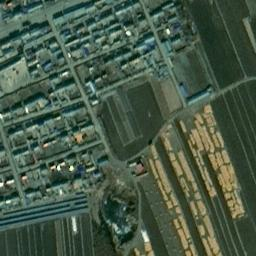
\includegraphics[width=\textwidth]{example/e1c.jpg}
	\end{minipage}}
	\subfigure[标注]{
		\begin{minipage}[t]{0.28\linewidth}
			\centering
			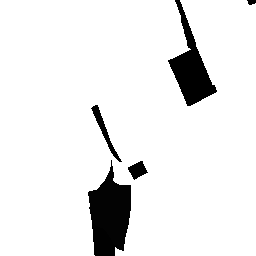
\includegraphics[width=\textwidth]{example/e1bw.png}
	\end{minipage}}

    \subfigure[训练集]{
		\begin{minipage}[t]{0.28\linewidth}
			\centering
			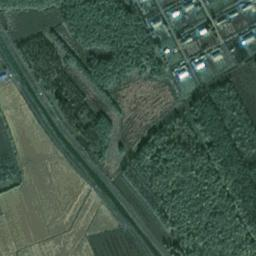
\includegraphics[width=\textwidth]{example/e2c.jpg}
	\end{minipage}}
	\subfigure[标注]{
		\begin{minipage}[t]{0.28\linewidth}
			\centering
			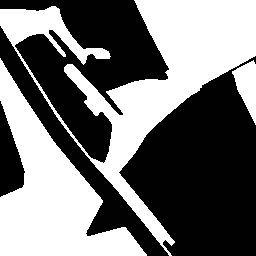
\includegraphics[width=\textwidth]{example/e2bw.png}
	\end{minipage}}
	
\end{figure}

\part{设计思路}

\chapter{设计概述}
Transfomer是一种在自然语言处理领域中流行的模型。近年来,Transfomer的成功
为涉及全局关系的深度学习领域的研究提供了新的方法。Visual Transfomer (ViT)\cite{vit}将Transfomer
引入计算机视觉领域,获得了良好效果。基于ViT的语义分割\cite{segmenter}在ADE20K数据集上
达到State-of-the-art,超越了其他同类模型。Swin Transfomer\cite{swin}通过构建
层次化的Transformer改进了ViT,并且引入Locality,在ADE20K数据集上达到了53.5的mIOU。
因此在语义分割任务上,Swin Transformer是一种极具前景的主干网络,有很好的效果预期。

\begin{figure}[htbp]
    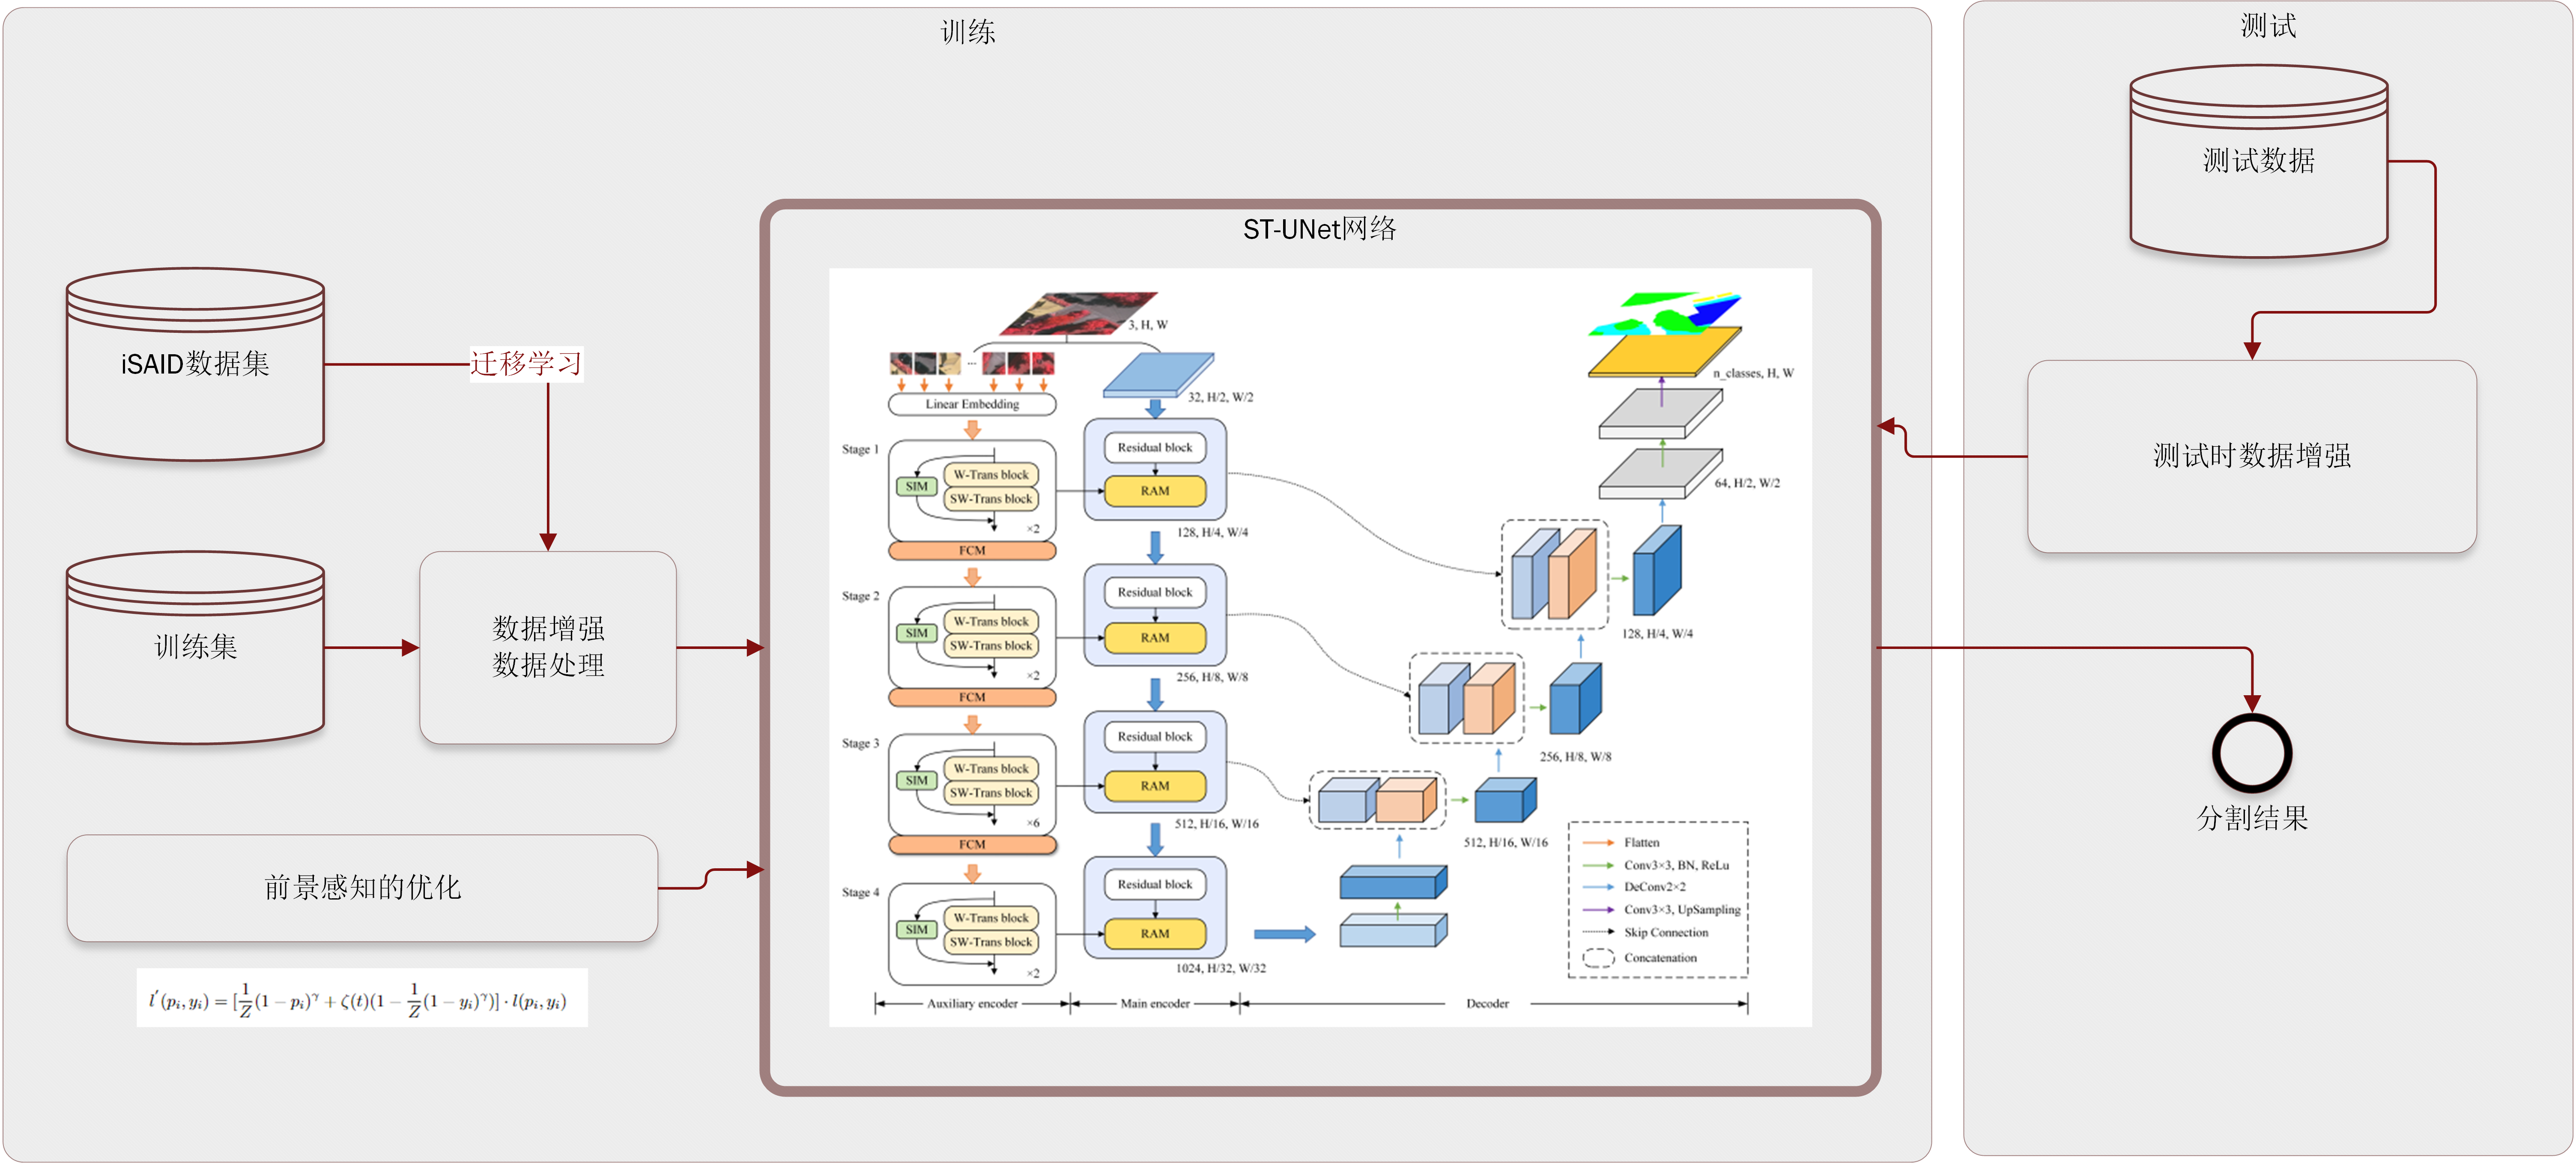
\includegraphics[width=\textwidth]{flowchart.png}
    \centering
    \caption{整体设计}
    \label{fig:fulldesign}
\end{figure}

图~\ref{fig:fulldesign}是我们的整体设计示意图。我们计划使用通过混合CNN和Swin Transformer结构在遥感影像语义分割上取得了良好效果的
\emph{嵌入了Swin Transformer的UNet(ST-UNet)}\cite{stunet}作为网络结构进行调整和训练。
该网络结构融合了Swin Transformer和有成熟广发应用的CNN结构,可以期望能达到
较好的效果。

为了处理遥感图像分割中样本的不均衡问题,尤其是前景-背景的不均衡问题,我们计划试验使用
FarSeg\cite{farseg}中提出的\emph{前景感知的优化},即使用损失函数\eqref{eqn:newloss}

\begin{equation}
    \label{eqn:newloss}
    l^{'}(p_i,y_i)=[\frac{1}{Z}(1-p_i)^\gamma+\zeta (t)(1-\frac{1}{Z}(1-y_i)^\gamma)]\cdot l(p_i,y_i)
\end{equation}

通过以背景中的困难部分作为权重较高的部分,可以是网络集中在前景和背景中的困难样本中,从而实现均衡优化。

Transformer主干网络的模型通常相对于CNN为主干网络的模型难以训练。为了解决这个问题,我们将应用\emph{迁移学习}的方法。
考虑到题目给定的数据集尺寸相对较小,我们首先从预训练模型开始,先在更大更完全的遥感影像数据集中预训练该网络,然后再在题目
给定的数据集中进行训练。这是提高准确性的有效方法。我们计划采用iSAID数据集\cite{isaid},该数据集提供了2806张遥感影像,来自
有多种传感器和多分辨率的平台,图像大小从$800\times800$到$4000\times13000$不等。为了使得该数据集
和题目给定的数据集尽可能接近,我们将会对iSAID数据集进行进一步处理,裁切成$256\times256$的分块。

在数据处理方面,我们将对遥感影像进行\emph{数据增强},包括随机裁剪、亮度,对比度和饱和度的调整
加入噪点与随机模糊等。这些影像变换可以模拟遥感图像采集中常见的图像缺陷。这些缺陷可能干扰识别,通过
对训练集进行数据增强,可以降低这些负面因素对网络训练的影响。

为了保证采取的各项措施行之有效、对模型的性能提升有实际作用,我们将进行\emph{消融试验}(Ablation Study),
对各种措施的不同组合分别进行测试并对性能参数进行统计,依据统计结果对措施的参数进行调整,或者确定移除某项措施,
或者添加某项措施,力求保证各措施有效,措施之间没有相互拮抗的现象发生。

在模型实际应用的过程中,我们将会应用\emph{测试时增强}的方法,在测试时通过数据增强产生额外的推理结果
在此基础上进行投票可以获得更好的性能表现。


\chapter{整体设计}

\section{遥感图像分割任务与ST-UNet}
遥感影响的物体分割是一种语义分割任务。这种任务面对大规模的变化、大规模的类内背景差异和较大的类外背景差异。
以及前景-背景不平衡的问题。一般的语义分割常常更加关注自然场景中的尺度变化,而没有充分地考虑到其他的问题\cite{farseg}。
并且常见的CNN作为主干网络的模型由于卷积运算的局部性,难以对网络的全局特征进行直接获取。

Swin Transformer在实践中展现出了极为强大的全局建模能力。而UNet是一种常用、表现优秀的的语义分割框架。因此将Swin Transformer嵌入传统的基于CNN的UNet
中,可以得到ST-UNet这一融合的遥感图像语义分割的框架\cite{stunet},它具有Swin Transformer
和CNN平行工作的\emph{双Encoder}架构。一方面,ST-UNet使用空间交互模块(Spatial Interation Module, STM)通过Swin Transformer编码像素级
的相关性来提高特征的代表能力,尤其是\emph{受到遮蔽的物体}。另一方面,该模型通过一个特征压缩模块(Feature Compression Module, FPM)来减少
详细信息的丢失,并在补丁标记下采样时浓缩更多的小规模的特征,这些小尺度的特征可以提高地面小尺度物体的分割精度。

最后,作为以上两个编码器的桥梁,该网路通过一个关系聚合模块(Relation Aggregation Module, RAM)来聚合两个编码器的特征,将Swin Transformer获得的全局相关关系
层级化地集成到CNN中。这种方式对在真实世界数据集中的识别起到了极为显著的提高\cite{stunet}。

在该方案中,我们采用该网络的原因主要有如下两点

\begin{itemize}
    \item Transformer框架在计算机视觉领域有良好的前景
    \item ST-UNet表现出了较好的性能
\end{itemize}


\section{前景感知的优化}
前景感知的优化是\cite{farseg}中提出了重要优化之一。前景与背景不均衡的问题常常导致在训练过程中背景主导了梯度,
但是只有北京的困难部分队训练后期的优化有价值,而这些样本相对稀少。这是该优化提出的动力。它的核心是将损失函数换成
\eqref{eqn:newloss2},借此将网络集中在前景和背景的困难样本上。

\begin{equation}
    \label{eqn:newloss2}
    l^{'}(p_i,y_i)=[\frac{1}{Z}(1-p_i)^\gamma+\zeta (t)(1-\frac{1}{Z}(1-y_i)^\gamma)]\cdot l(p_i,y_i)
\end{equation}

其中$p_i$是预测的概率,$y_i$代表第$i$像素的Ground truth。$Z$是一个归一化常数,该常数保证$\sum l(p_i,y_i)=\frac{1}{Z}\sum(1-p_i)^\gamma l(p_i,y_i)$。
$l(p_i,y_i)$是一个交叉熵损失函数。$\zeta(t)$是一个单调递减的退火函数,其取值范围在$[0,1]$之间。有线性、多项式、余弦三种选择,如图~\ref{fig:annel_func},
每种选择有各自的超参数可供控制和调整。

\begin{figure}[htbp]
    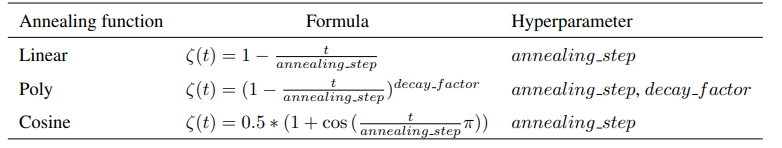
\includegraphics[width=\textwidth]{annealing_funcs.png}
    \centering
    \caption{退火函数}
    \label{fig:annel_func}
\end{figure}

虽然该优化和主干网络ST-UNet并不来源于同一个工作,但是该优化对遥感图像分割任务中有显著影响的不均衡问题提出了
解决方案,该解决方案与主干网络独立,具有一定的普适性。因此将该优化加入ST-UNet中以测试其性能并作为一种
可能的优化候选是合理的,一定程度上也是必要的。

\section{迁移学习}

尽管Transformer在图像上的应用具有较强的竞争力,但是与成熟的卷积神经网络相比,训练技巧还并不成熟\cite{howtotrain},
并且由于参数量的区别,Transformer训练通常较难。因此,本方案对ST-UNet的训练将使用预训练模型进行迁移学习。

迁移学习是通过从预训练网络开始训练来获得更好的结果的一种方法。迁移学习背后的理念是如果一个
模型基于足够大且通用的数据集训练的,那么该模型将有效地充当视觉世界的通用的模型。随后,这些学习到的
特征映射可以被重用,而不必通过从头开始的方式训练。

迁移学习具有相当的重要性重要性。这是因为\cite{howtotrain}中提到,就大多数实际目的而言,迁移预先训练的模型不仅成本效益较高,
而且会带来更好的结果。对于类似题目所给的这样数据量相对同邻域常用数据集较小的数据集而言,几乎不可能
通过从零开始训练使其达到接近迁移模型的精度。而对于足够大的数据集,从零开始达到与迁移模型相似的精度
则需要多花超过2个数量级的时间。


\section{数据增强}

遥感图像分割任务本身的性质决定了该模型需要面对多变的、不均衡的数据。为了在训练阶段能够更好地提高模型
的识别能力,需要对数据集进行增强。首先,就训练用的遥感图像,我们初步计划进行以下的增强
\begin{itemize}
    \item \textbf{几何变换} 几何变换包括随即旋转、随机缩放、随机镜像翻转等变换,这些变换可以代表遥感图像产生过程中的角度差异。
    \item \textbf{色彩变换} 包括随机改变亮度、对比度、饱和度等参数,这些是图常见的差异,但这些差异不应当对分割结果造成过大的影响。
    \item \textbf{噪声} 噪声包括随机噪声、随机模糊、随机拼接色差、随机条带等。可以模拟真实世界中遥感图像的缺陷。
\end{itemize}
在测试时,本方案将进行测试时数据增强。测试时主要对遥感图像进行几何变换,例如
\begin{itemize}
    \item 水平、垂直翻转
    \item 旋转
\end{itemize}
并采用逐像素少数服从多数的投票法进行硬投票,应当可以增加结果的准确性。

此外,当数据集不能完全满足需求时,可以采用GAN\cite{ganaug}生成数据。但该方案在实际使用中可能出现
生成质量不高等问题,是一个备用的方案。

此外,从Transformer的性质出发,还有一些常用的增强方法,如Mixup\cite{mixup}、CutMix\cite{cutmix}、
RandAugment\cite{randaug}等。这些增强方法也是必要的。

\part{实现方法}

\chapter{模型实现}

\section{主干网络和前景感知的优化}

\begin{figure}[htbp]
    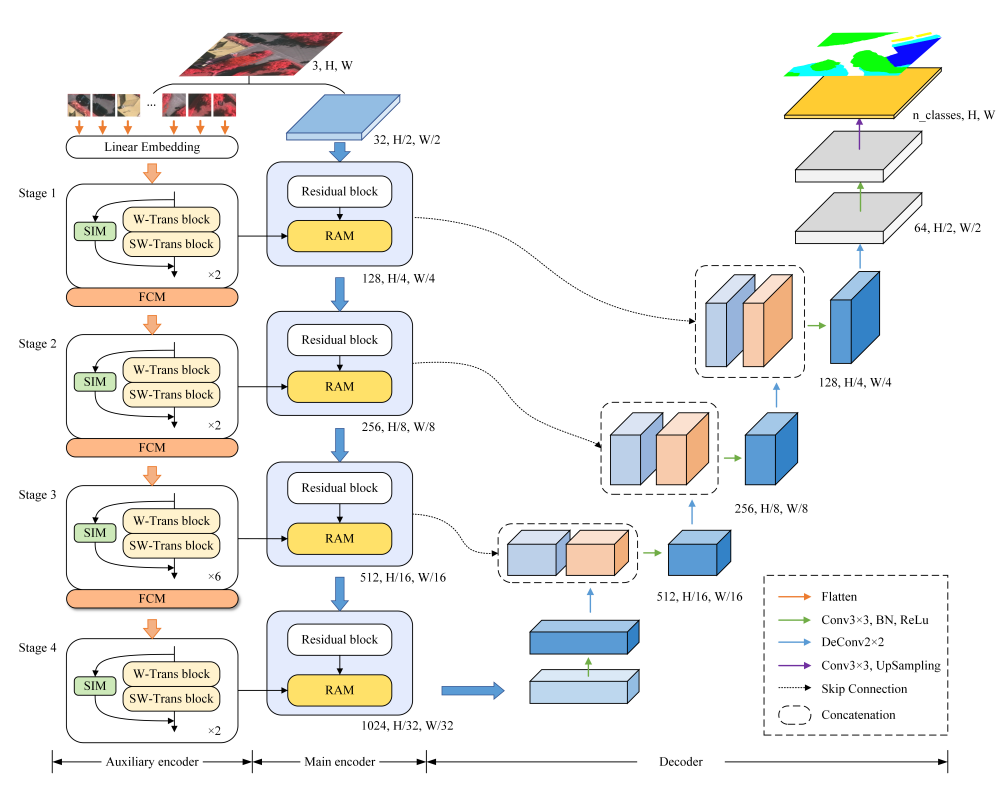
\includegraphics[width=\textwidth]{net_arch.png}
    \centering
    \caption{网络结构}
    \label{fig:netarch}
\end{figure}

ST-UNet的整体架构如图~\ref{fig:netarch}。它有UNet和Swin Transformer的混合i二狗
该结构保留了UNet的跨编码器-解码器连接的优秀特点。特别地,该结构有一个双编码器架构,
该架构由Swin Transformer和基于CNN的残差连接网路组合而成,然后通过RAM完全获得遥感影像的
信息,然后由SIM和FCM进行处理,这个过程可以显著地提高模型的表现。这些模块的结构如图~\ref{fig:netsimfcmram}。


该模型的论文\cite{stunet}中提供了开源代码地址。该开源实现是一个基于pyTorch的实现。考虑的pyTorch
与PaddlePaddle的API有相当大的相似性,同时PaddlePaddle提供了和pyTorch相对应的API对照表,因此
该实现可以轻松地迁移到PaddlePaddle,构成本方案的主干网络。

\begin{figure}[H]
    \centering
	\caption{SIM模块、FCM模块和RAM模块}
	\label{fig:netsimfcmram}
	
	\subfigure[SIM]{
		\begin{minipage}[t]{0.32\linewidth}
			\centering
			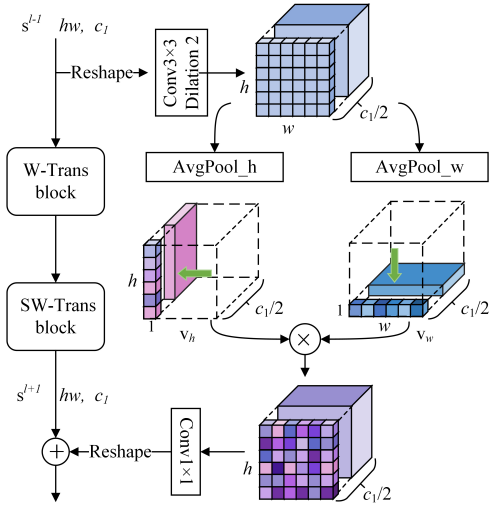
\includegraphics[width=\textwidth]{sim.png}
	\end{minipage}}
	\subfigure[FCM]{
		\begin{minipage}[t]{0.48\linewidth}
			\centering
			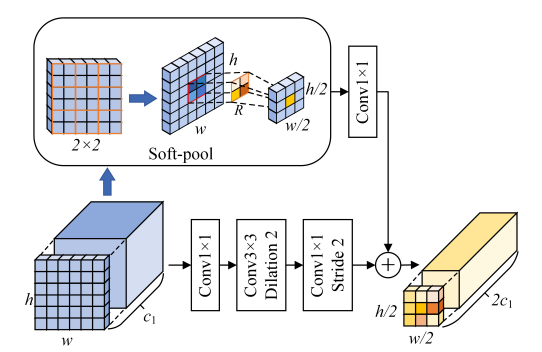
\includegraphics[width=\textwidth]{fcm.png}
	\end{minipage}}

    \subfigure[RAM]{
		\begin{minipage}[t]{0.8\linewidth}
			\centering
			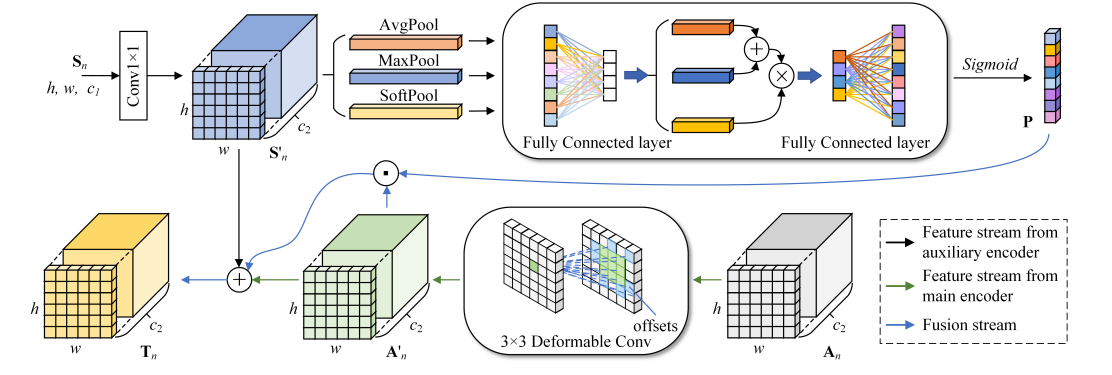
\includegraphics[width=\textwidth]{ram.png}
	\end{minipage}}
	
\end{figure}


前景感知的优化主要是实现损失函数\eqref{eqn:newloss2}。该实现较为容易,并且FarSeg有开源实现,可以
通过对\url{https://github.com/Z-Zheng/FarSeg/blob/master/module/loss.py}进行简单的修改从而
实现。

\begin{lstlisting}[language=Python,numbers=left,style=PythonStyle,label={code:loss},caption=前景感知的优化中损失函数的实现]
def annealing_softmax_focalloss(y_pred, y_true, t, t_max, ignore_index=255, gamma=2.0,
                                annealing_function=cosine_annealing):
    losses = F.cross_entropy(y_pred, y_true, ignore_index=ignore_index, reduction='none')
    with torch.no_grad():
        p = y_pred.softmax(dim=1)
        modulating_factor = (1 - p).pow(gamma)
        valid_mask = ~ y_true.eq(ignore_index)
        masked_y_true = torch.where(valid_mask, y_true, torch.zeros_like(y_true))
        modulating_factor = torch.gather(modulating_factor, dim=1, index=masked_y_true.unsqueeze(dim=1)).squeeze_(dim=1)
        normalizer = losses.sum() / (losses * modulating_factor).sum()
        scales = modulating_factor * normalizer
    if t > t_max:
        scale = scales
    else:
        scale = annealing_function(1, scales, t, t_max)
    losses = (losses * scale).sum() / (valid_mask.sum() + p.size(0))
    return losses
\end{lstlisting}

该文件中$*\_annealing$是退火函数的实现,而$annealing\_softmax\_focalloss$是式\eqref{eqn:newloss2}
的代码实现,在这里给出如代码~\ref{code:loss}。可以发现该实现只依赖于少数的用于交叉熵损失和生成张量的pyTorch API,因此迁移到PaddlePaddle
是相当容易的。

\section{数据增强}

数据增强中对图像的几何变换和色彩变换可以简单地使用numpy的基本操作和sklearn等库进行实现。
这里主要介绍其余几种较为复杂的数据增强方法的实现。

\subsection{Mixup}

Mixup\cite{mixup}是一种相对简单的数据增广策略,通过对输入数据进行简单的线性变换\eqref{eqn:mixup}

\begin{equation}
    \label{eqn:mixup}
    \widetilde{\bvec{X}}=\lambda\cdot\bvec{X_0}+(1-\lambda)\cdot\bvec{X_1}
\end{equation}
可以有效地增加模型的泛化能力,并且能提高模型对于对抗攻击的鲁棒性。其中$\lambda$取自$\beta$分布,可以取
$\lambda \sim \beta(2,2)$,使得$\lambda$的取值范围在0.5附近。这样可以取得更好的效果。\url{https://github.com/hongyi-zhang/mixup/blob/master/cifar/utils.py}
中提供了一个Mixup的实现,同样易于迁移到PaddlePaddle。

\subsection{CutMix}
CutMix\cite{cutmix}是一种通过拼接图像来进行正则化的数据增强方法,它的定义的是\eqref{eqn:cutmix}
\begin{equation}
    \label{eqn:cutmix}
    \begin{aligned}
        \widetilde{x}&=\bvec{M}\odot x_A+(\bvec{1}-\bvec{M})\odot x_B \\
        \widetilde{y}&=\lambda\cdot y_A+(1-\lambda)\cdot y_B 
    \end{aligned}
\end{equation}
其中$\bvec{M}$是一个二进制掩码。该策略相当于对图像随机剪裁之后硬混合,并对标签进行线性组合。$\bvec{M}$
的取法常常从图像的长款中进行均匀分布的随机取样,即
\begin{equation}
    \label{eqn:cutmix_mask}
    \begin{aligned}
        r_x &\sim U(0,W),\ r_w=W\sqrt{1-\lambda} \\
        r_y &\sim U(0,H),\ r_h=H\sqrt{1-\lambda} \\
    \end{aligned}
\end{equation}
该策略较为简单直观,也可以通过现有开源库的组合进行实现。

\subsection{RandAugment}

RandAugment\cite{randaug}是谷歌提出的一种解决自动化增强搜索空间巨大、无法针对具体的模型
和数据大小的问题的方法。谷歌给出的实现是代码~\ref{code:randaug}。

\begin{lstlisting}[language=Python,numbers=left,style=PythonStyle,label={code:randaug},caption=RandAugment]

import numpy as np

transforms = ['Identity', 'AutoContrast', 'Equalize', 'Rotate', 'Solarize', 'Color', 'Posterize', 'Contrast',
              'Brightness', 'Sharpness', 'ShearX', 'ShearY', 'TranslateX', 'TranslateY']

def randaugment(N, M):
    '''
    Generate a set of distortions.
    Args:
    N: Number of augmentation transformations to
    apply sequentially.
    M: Magnitude for all the transformations.
    '''
    sampled_ops = np.random.choice(transforms, N)
    return [(op, M) for op in sampled_ops]

\end{lstlisting}

该方法简单直观:随机从大量的变换类型中选择$N$种,并且以强度$M$返回这些变换。
之后可以对该$M\cdot N$大小的搜索空间进行网格搜索,得到最优的增强策略。这种方法
并不逊色于PBA、FastAA等数据增强方法,并且显著地减少了搜索空间\cite{ganaug},
在多数网络上有较好的效果。

\chapter{训练与测试}

测试和调整是非常重要的一步。该部分实现流程主要如图~\ref{fig:modeltraining}
我们将使用消融试验和参数搜索等方法优化我们的模型。

\begin{figure}[htbp]
    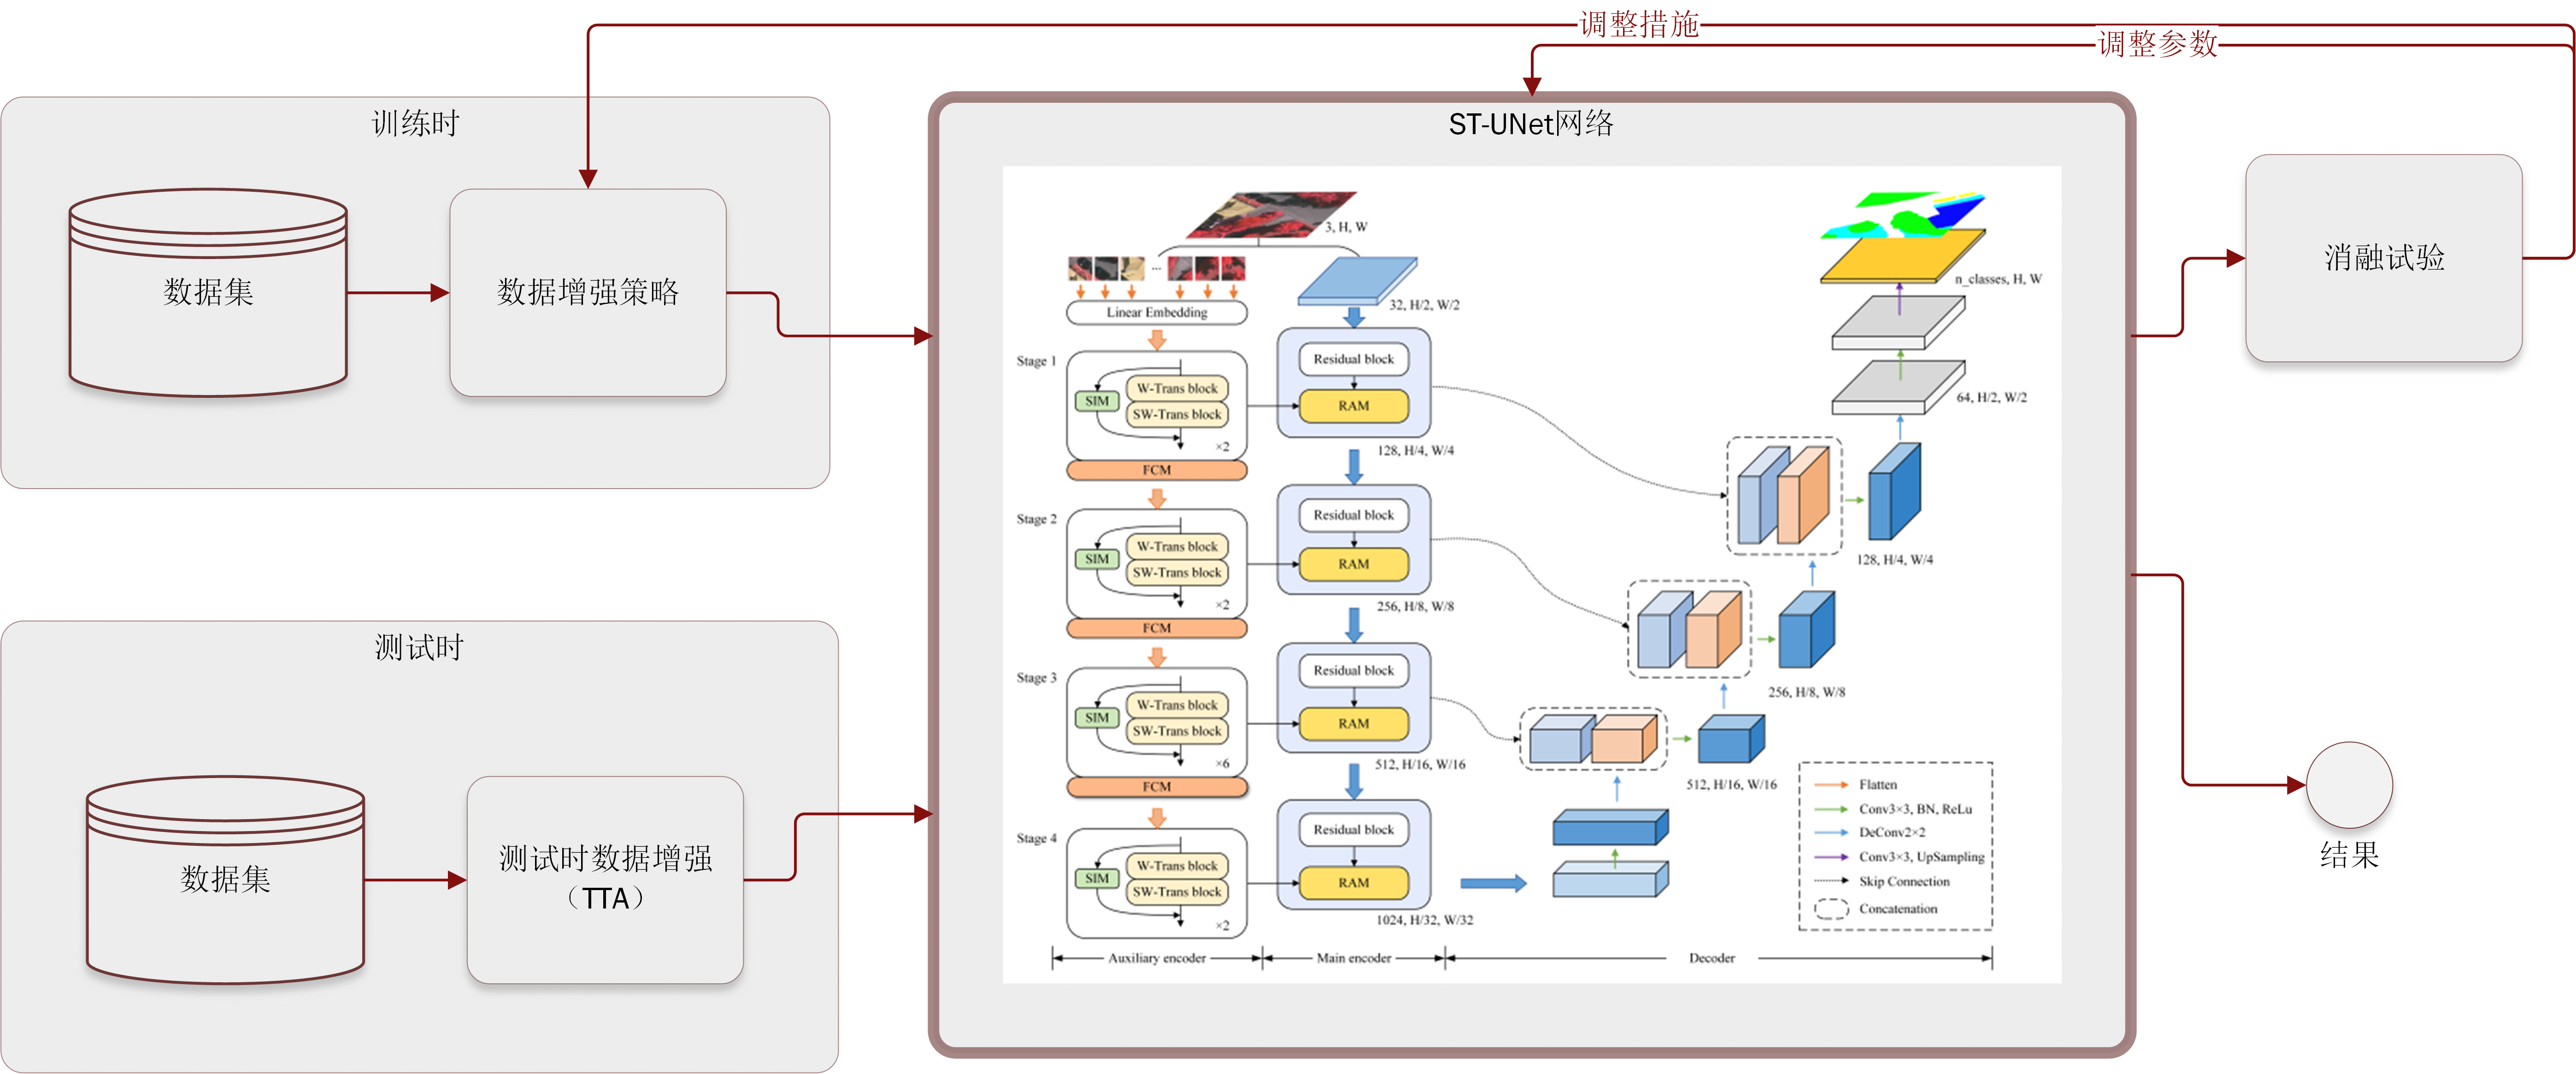
\includegraphics[width=\textwidth]{model.png}
    \centering
    \caption{训练和测试}
    \label{fig:modeltraining}
\end{figure}

\section{训练方法}
本方案选择了Transformer的网络结构。Transformer有较为难以训练的特点,因此我们采用
AdamW优化器。AdamW常常用于大型预训练模型。它是对Adam优化器的一个改进,为Adam优化器加入L2正则
使得参数值不会太大。这种方式可以缓解过拟合的问题。此外,训练轮次将使用较大的数值,如300以上。
在训练时,首先加载预训练模型的参数,通过迁移学习的方法提高模型的准确性。整体训练过程的Pipeline
如图~\ref{fig:trainpipe}所示。

\begin{figure}[htbp]
    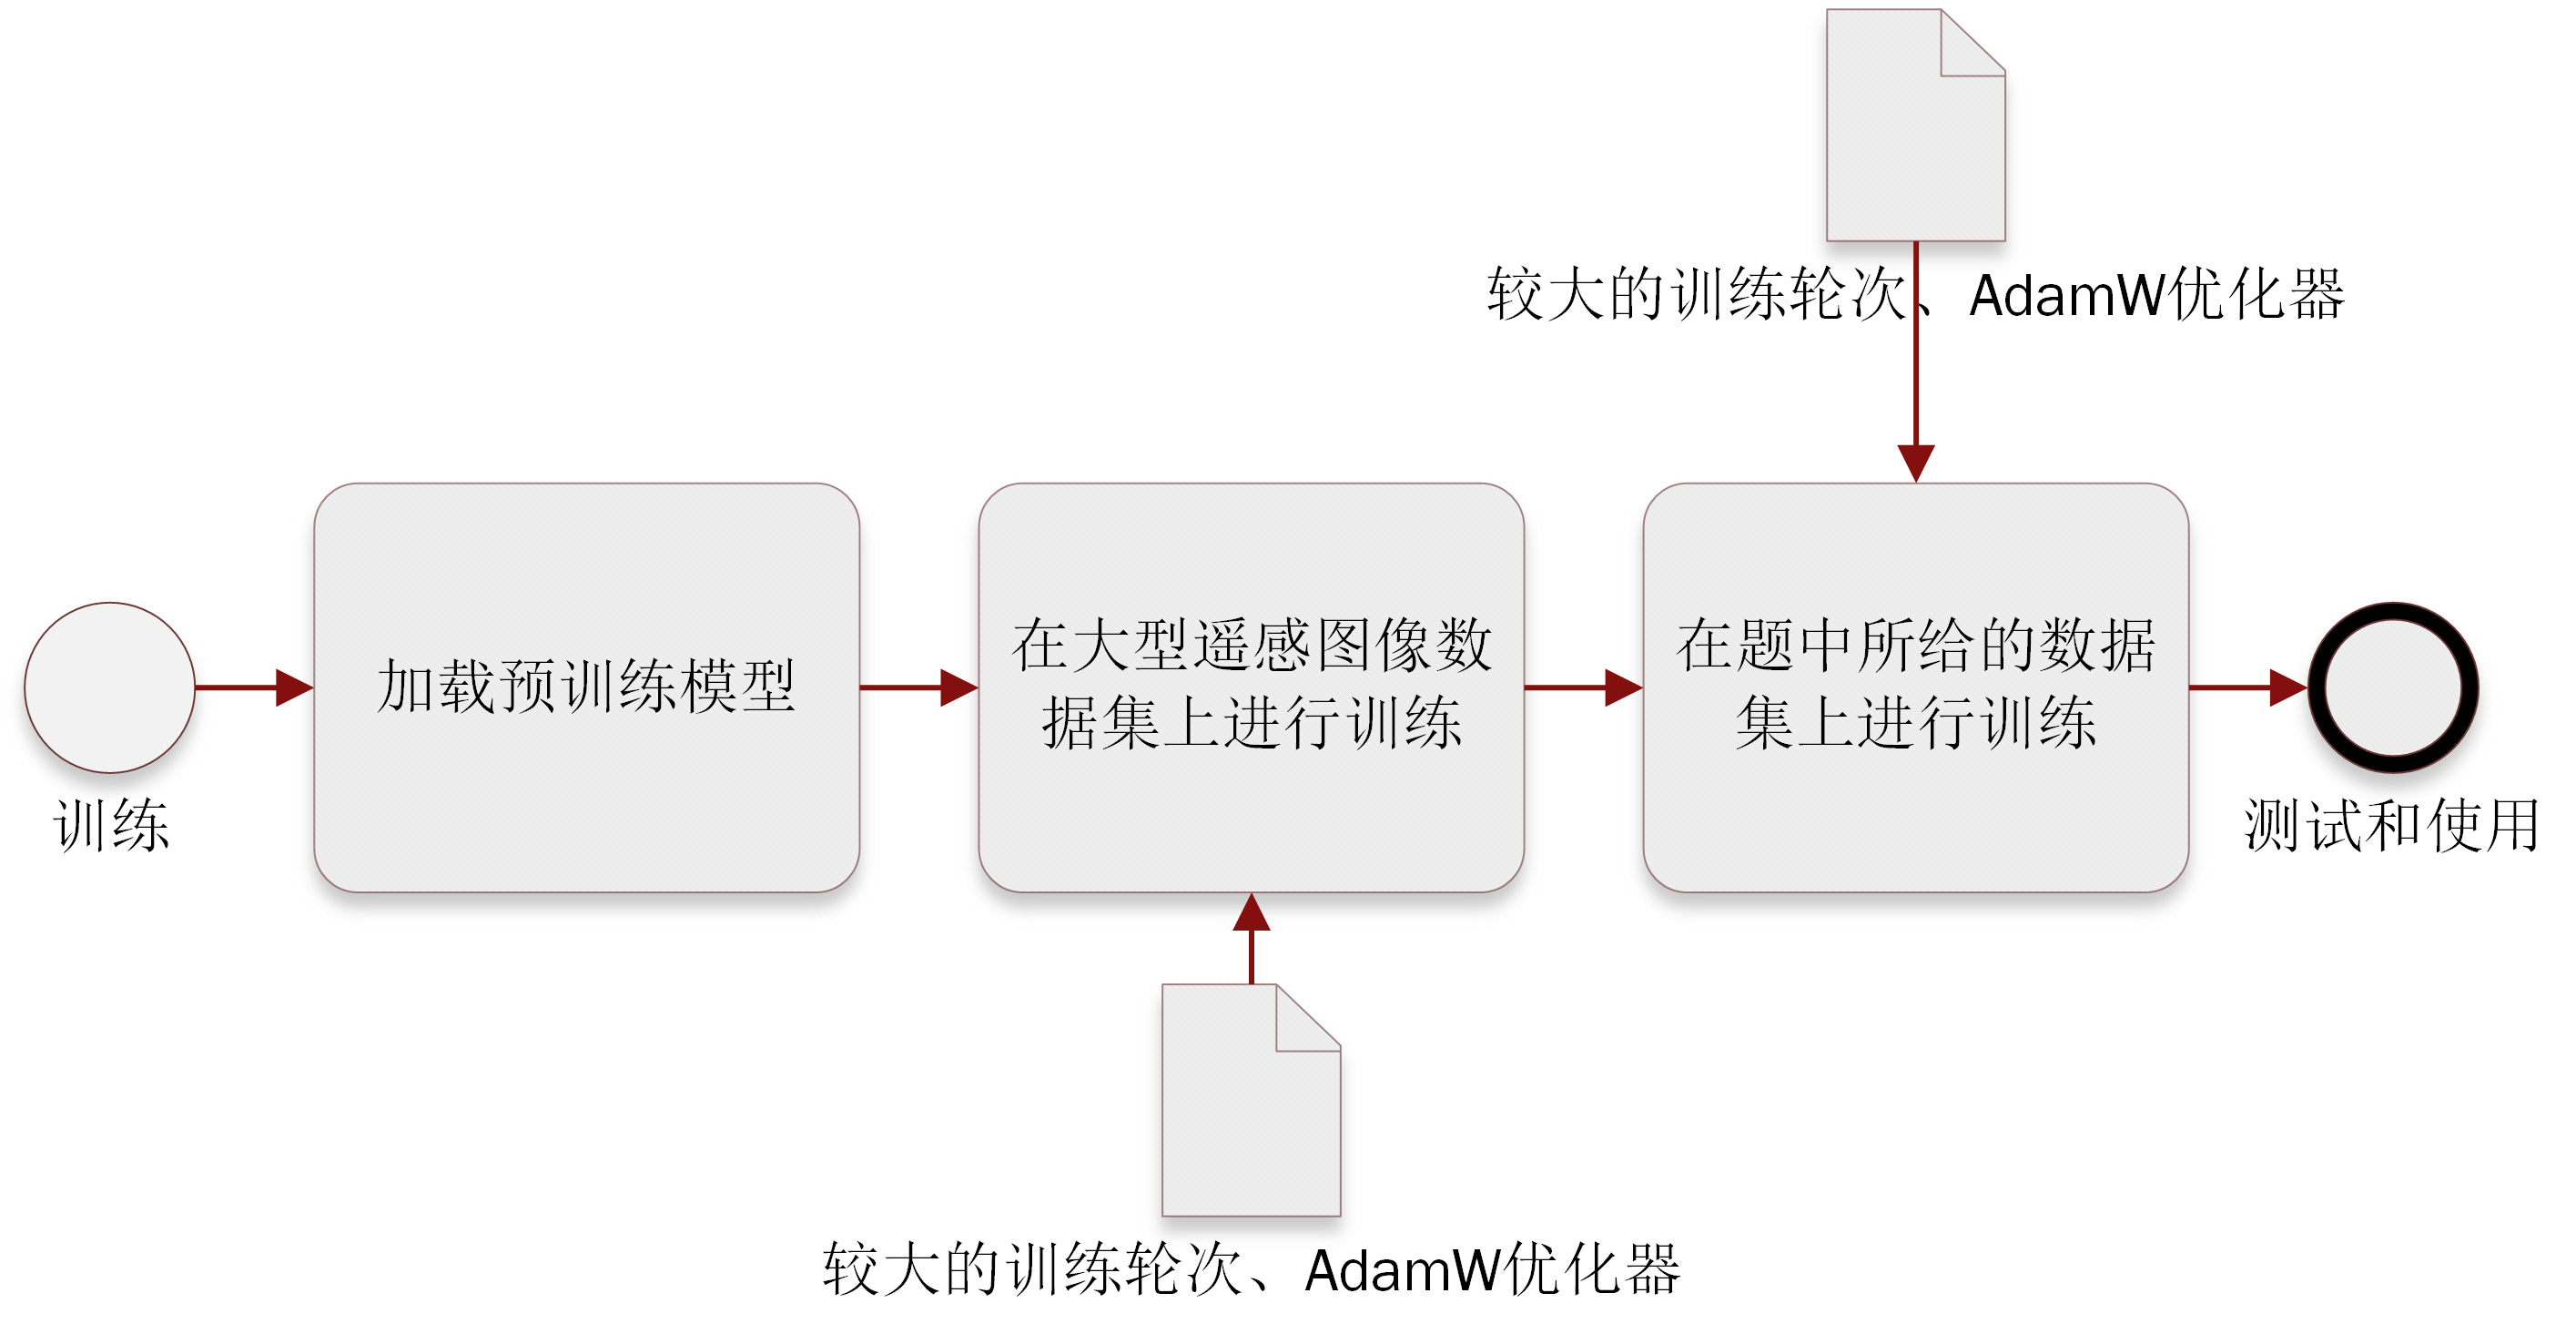
\includegraphics[width=\textwidth]{train.png}
    \centering
    \caption{训练流程}
    \label{fig:trainpipe}
\end{figure}

参照不同Transformer的训练方法及\cite{howtotrain}的结论,在训练中需要的各种参数设计如表~\ref{tbl:train},
这些参数将会根据实践的效果进行调整,以达到更好的效果。

\begin{table}[htbp]
    \centering
    \caption{训练参数}
    \label{tbl:train}
    \renewcommand\arraystretch{1.5}
    \begin{tabular}{c|c}
        \toprule
        \hline
        参数 & 值 \\
        \hline
        优化器 & AdamW \\
        训练轮次(Epochs) & 300/300 \\
        每轮训练数据量(Batch Size) & 64/32 \\
        训练策略 & 早停、学习率衰减 \\
        \hline
        \bottomrule
    \end{tabular}
\end{table}

\section{消融试验}

消融试验是一种常用的方法,为了检验采取多项改进时每一项改进都对效果的提高具有正向贡献,
需要对各项改进单独出现、成组出现的情况进行测试。由于本方案为了有效地进行遥感图像语义分割进行了多项措施,
为了检验各项措施,我们将进行消融试验,并依照试验结果进行评估,对措施进行重新调整,试验计划如表~\ref{tbl:ablexpr}。

\begin{table}[htbp]
    \centering
    \caption{消融试验计划}
    \label{tbl:ablexpr}
    \renewcommand\arraystretch{1.5}
    \begin{tabular}{ccc|c}
        \toprule
        \hline
        前景感知的优化 & 额外数据集的迁移学习 & 数据增强 & mIOU\\
        \hline
        $\checkmark$ & \ & \ & 待测 \\
        \ & $\checkmark$ & \ & 待测  \\
        \ & \ & $\checkmark$ & 待测  \\
        $\checkmark$ & $\checkmark$ & \ & 待测  \\
        $\checkmark$ & \ & $\checkmark$ & 待测  \\
        \ & $\checkmark$ & $\checkmark$ & 待测  \\
        $\checkmark$ & $\checkmark$ & $\checkmark$ & 待测 \\
        \hline
        \bottomrule
    \end{tabular}
\end{table}

我们期望在消融试验中得到性能参数逐次增高的效果。如果某项措施的效果不能达到预期的效果,
我们会考虑
\begin{itemize}
    \item 对该项措施进行重新调整;
    \item 移除该项措施
\end{itemize}
然后重新进行测试并评估效果。

\part*{参考文献}
\addcontentsline{toc}{part}{参考文献}

\bibliographystyle{unsrt}
\bibliography{reference}

\end{document}